\documentclass[document.tex]{subfiles} 
\begin{document}

\clearpage

\subsection{Мультиплексоры и демультиплексоры}
Mультиплексор -- устройство, имеющее несколько сигнальных входов, один или более
управляющих входов и один выход. Мультиплексор позволяет передавать сигнал с
одного из входов на выход; при этом выбор желаемого входа осуществляется подачей
соответствующей комбинации управляющих сигналов. Устройство, противоположное
мультиплексору по своей функции, называется демультиплексором~\cite{wikimux}.

Вся кодовая база мультиплексоров и демультиплексоров находится в пакете
devices.mux и наследуется от абстрактного класса Device. 

\clearpage
\subsubsection{Mультиплексор}

Mультиплексор можно описать следующим образом:
\begin{equation}
\label{eq:mux}
\forall x: (D_x = 1) \wedge (A = x) \Leftrightarrow (O_0 = 1)
\end{equation}

В выражении~\ref{eq:mux}:
\begin{itemize}[noitemsep]
  \item $x$ -- индекс входного разряда данных;
  \item $D$ -- набор входных разрядов данных;
  \item $A$ -- набор входных разрядов адреса;
  \item $O_0$ -- выходной разряд.
\end{itemize}

Описание мультиплексора в разрабатываемой библиотеке представлено в
листинге~\ref{lst:mux}.

\begin{listing}[ht]
\begin{minted}[linenos=true]{python}
class DeviceMux(Device):
    """Multiplexer device"""
    mandatory_signals = ('strobe_signals', 'address_signals',
                         'data_signals', 'output_signals',)
    mandatory_signals_using_subs = ('strobe_signals', 'output_signals',)
    truth_table_signals = ('strobe_signals', 'address_signals',
                           'data_signals', 'output_signals',)
    constraints = {
        'strobe_signals': {
            'min': 1,
            'max': 10
        },
        'address_signals': {
            'min': 1,
            'max': 5
        },
        'data_signals': {
            'min': 1,
            'max': 32
        },
        'output_signals': {
            'min': 1,
            'max': 1
        }
    }
\end{minted}
\caption{Программное описание класса мультиплексора}
\label{lst:mux}
\end{listing}

\clearpage
В листинге~\ref{lst:muxgen} представлен код для программного синтеза
мультиплексора с 4 входными разрядами данных (data\_signals='d:4'), 2 входными
разрядами адреса (address\_signals='a:2'), 1 прямым входным разрядом
строб-сигнала (strobe\_signals='z:1') и 1 прямым выходным разрядом
(output\_signals='o:1').

\begin{listing}[ht]
\begin{minted}{pycon}
>>> from circuitry.devices.mux import DeviceMux        
>>> pprint(                                               
...     DeviceMux(strobe_signals='z:1', address_signals='a:2',
...               data_signals='d:4', output_signals='o:1',
...               strobe_signals_subs=dict(z0=1),
...               output_signals_subs=dict(o0=1))
... )
{'address_and_data_function': Or(And(Not(a0), Not(a1), Not(d1), 
                              Not(d2), Not(d3), d0), And(Not(a0), 
                              Not(d0), Not(d1), Not(d3), a1, d2), 
                              And(Not(a1), Not(d0), Not(d2), Not(d3), a0, d1), 
                              And(Not(d0), Not(d1), Not(d2), a0, a1, d3)),
 'address_signals': (a0, a1),
 'data_signals': (d0, d1, d2, d3),
 'functions': [And(Or(
                      And(Not(a0), Not(a1), Not(d1), Not(d2), Not(d3), d0),
                      And(Not(a0), Not(d0), Not(d1), Not(d3), a1, d2),
                      And(Not(a1), Not(d0), Not(d2), Not(d3), a0, d1),
                      And(Not(d0), Not(d1), Not(d2), a0, a1, d3)), z0)
              ],
 'output_signals': (o0,), 
 'output_signals_function': o0, 
 'output_signals_subs': {'o0': 1}, 
 'output_signals_truth_table': [1],
 'strobe_signals': (z0,), 'strobe_signals_function': z0,
 'strobe_signals_subs': {'z0': 1},
 'strobe_signals_truth_table': [1],
 'truth_table': [([1], [0, 0], [1, 0, 0, 0], [1]),
                 ([1], [1, 0], [0, 1, 0, 0], [1]),
                 ([1], [0, 1], [0, 0, 1, 0], [1]),
                 ([1], [1, 1], [0, 0, 0, 1], [1])]}
\end{minted}
\caption{Программный синтез мультиплексора}
\label{lst:muxgen}
\end{listing}

\clearpage

На рисунке~\ref{fig:devicemux} представлено условно-графическое обозначение
синтезированного мультиплексора.

\begin{figure}[here]
\centering
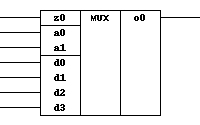
\includegraphics{devices_mux_sym}
\caption{Условно-графическое обозначение мультиплексора}
\label{fig:devicemux}
\end{figure}

На рисунке~\ref{fig:devicemuxmat} представлено устройство
синтезированного мультиплексора в виде модели Simulink.

\begin{figure}[here]
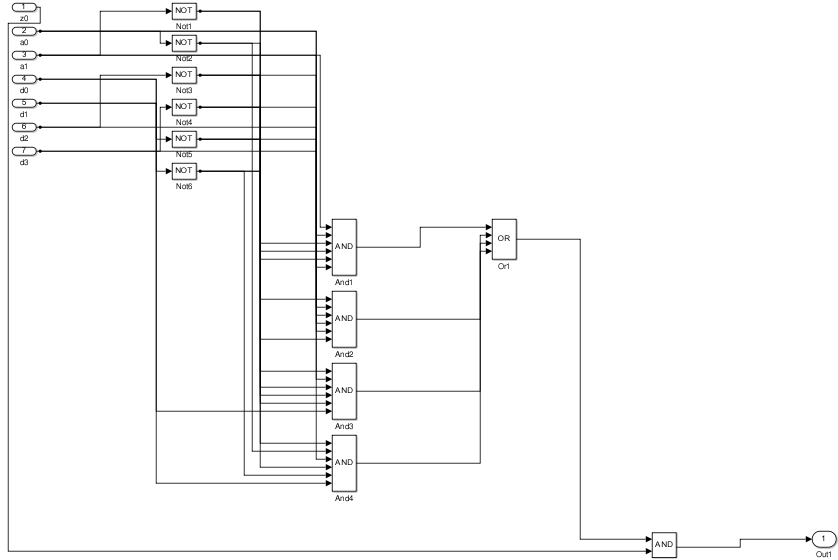
\includegraphics[width=1\linewidth]{devices_mux_mat}
\caption{Представление мультиплексора в виде модели Simulink}
\label{fig:devicemuxmat}
\end{figure}

\clearpage

\subsubsection{Демультиплексор}

Деультиплексор можно описать следующим образом:
\begin{equation}
\label{eq:demux}
\forall x: (D_0 = 1) \wedge (A = x) \Leftrightarrow (O_x = 1)
\end{equation}

В выражении~\ref{eq:demux}:
\begin{itemize}[noitemsep]
  \item $x$ -- индекс выходного разряда;
  \item $D_0$ -- входной разряд данных;
  \item $A$ -- набор входных разрядов адреса;
  \item $O$ -- набор выходных разрядов.
\end{itemize}

Описание демультиплексора в разрабатываемой библиотеке представлено в
листинге~\ref{lst:demux}.

\begin{listing}[ht]
\begin{minted}[linenos=true]{python}
class DeviceDemux(Device):
    """Demultiplexer device"""
    mandatory_signals = ('strobe_signals', 'address_signals', 
                         'data_signals', 'output_signals',)
    mandatory_signals_using_subs = ('strobe_signals', 'data_signals', 
                                    'output_signals')
    truth_table_signals = ('strobe_signals', 'address_signals', 
                           'data_signals', 'output_signals',)
    constraints = {
        'strobe_signals': {
            'min': 1,
            'max': 10
        },
        'address_signals': {
            'min': 1,
            'max': 5
        },
        'data_signals': {
            'min': 1,
            'max': 1
        },
        'output_signals': {
            'min': 1,
            'max': 32
        }
    }
\end{minted}
\caption{Программное описание класса демультиплексора}
\label{lst:demux}
\end{listing}

\clearpage

В листинге~\ref{lst:demuxgen} представлен код для программного синтеза
демультиплексора с 1 входным разрядом данных (data\_signals='d:1'), 2 входными
разрядами адреса (address\_signals='a:2'), 1 прямым входным разрядом
строб-сигнала (strobe\_signals='z:1') и 4 прямыми выходными разрядами
(output\_signals='o:4').

\begin{listing}[ht]
\begin{minted}{pycon}
>>> from circuitry.devices.mux import DeviceDemux        
>>> pprint(                                                     
...     DeviceDemux(strobe_signals='z:1', address_signals='a:2',
...                 data_signals='d:1', output_signals='o:4',
...                 strobe_signals_subs=dict(z0=1),
...                 data_signals_subs=dict(d0=1),
...                 output_signals_subs=dict(o0=1, o1=1, o2=1, o3=1))
... )
{'address_signals': (a0, a1),
 'data_signals': (d0,),
 'data_signals_function': d0,
 'data_signals_subs': {'d0': 1},
 'data_signals_truth_table': [1],
 'functions': [And(Not(a0), Not(a1), d0, z0),
               And(Not(a1), a0, d0, z0),
               And(Not(a0), a1, d0, z0),
               And(a0, a1, d0, z0)],
 'output_signals': (o0, o1, o2, o3),
 'output_signals_function': And(o0, o1, o2, o3),
 'output_signals_subs': {'o0': 1, 'o1': 1, 'o2': 1, 'o3': 1},
 'output_signals_truth_table': [1, 1, 1, 1],
 'strobe_signals': (z0,),
 'strobe_signals_function': z0,
 'strobe_signals_subs': {'z0': 1},
 'strobe_signals_truth_table': [1],
 'truth_table': [([1], [0, 0], [1], [1, 0, 0, 0]),
                 ([1], [1, 0], [1], [0, 1, 0, 0]),
                 ([1], [0, 1], [1], [0, 0, 1, 0]),
                 ([1], [1, 1], [1], [0, 0, 0, 1])]}
\end{minted}
\caption{Программный синтез демультиплексора}
\label{lst:demuxgen}
\end{listing}

\clearpage

На рисунке~\ref{fig:devicedemux} представлено условно-графическое обозначение
синтезированного демультиплексора.

\begin{figure}[here]
\centering
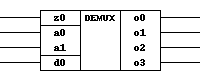
\includegraphics{devices_demux_sym}
\caption{Условно-графическое обозначение демультиплексора}
\label{fig:devicedemux}
\end{figure}

На рисунке~\ref{fig:devicedemuxmat} представлено устройство
синтезированного демультиплексора в виде модели Simulink.

\begin{figure}[here]
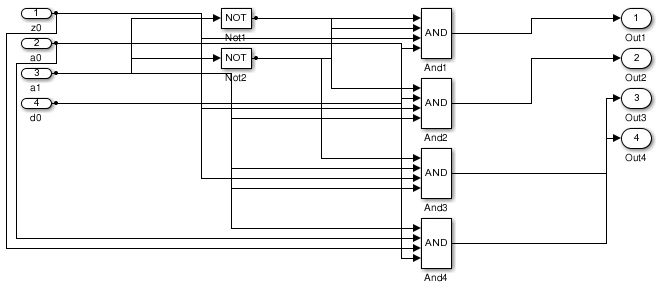
\includegraphics[width=1\linewidth]{devices_demux_mat}
\caption{Представление демультиплексора в виде модели Simulink}
\label{fig:devicedemuxmat}
\end{figure}

\end{document}